\section{Experiments}
\subsection{Setup}
\paragraph{Data.} We use the English \texttt{fortunes} collection, i.e.\ the data files of the Debian
\texttt{fortunes}/\texttt{fortunes-min} packages, excluding \texttt{ascii-art} and attribution lines.
It is lower-cased and mapped to $V=32$ symbols (\texttt{a--z}, space, \texttt{.\,,\,'\,?\,!}). Entries are
shuffled and split 90/5/5, giving $2.01\times10^6$ training, $1.19\times10^5$ validation and
$1.09\times10^5$ test characters. The unigram entropy is $4.26$~bits.
\paragraph{Models.} All local denoisers share the featuriser of Sec.~3.3 ($F=6{,}831$ sparse
features, 17 active per position). They differ only in the read-out. \emph{Log-linear softmax}: summed
feature logits with a per-$t$ logit scale (the classical analogue of $J(t)$). \emph{MLP softmax}: summed
240-dimensional feature embeddings, two GELU layers, softmax. \emph{Exchange (linear ctrl.)}: summed
pulse areas for $G=240$ exchange gates (butterfly, 3 blocks) with envelope $J(t)$. \emph{Exchange (MLP
ctrl.)}: the MLP above with a 240-angle output feeding the same circuit.
\paragraph{Training and evaluation.} Each run uses Adam \citep{kingma2015adam}, learning rate
$2\times10^{-3}$ (200-step warm-up, cosine decay), $10^4$ steps, and 64 windows of 64 characters per
step. Training is on CPU: about 25~minutes per exchange model on one core, using our real-arithmetic
simulator. We report the test NELBO in bits/char, summing $\mathcal L_{t-1}$ over \emph{all} $T=32$ steps
(no Monte-Carlo over $t$) on 256 test windows. For sample quality we draw 256 unconditional samples of
length 64 by measurement-based ancestral sampling. We score them by (a) their bits/char under an
interpolated Kneser--Ney 5-gram fitted to the training split \citep{chen1999empirical} and (b) the
fraction of interior words of length $\ge2$ that occur in the training vocabulary.

\subsection{Verification of the simulator and theory}
\begin{table}[t]
\centering\small
\caption{Numerical checks. Top: exact agreement of the single-excitation simulator with a full
$2^6$-dimensional Heisenberg simulation of a 4-layer chain, together with the identities used in
Secs.~3--4 (for $V=32$). Bottom: dimension of the dynamical Lie algebra generated by $\{iL_{ab}\}$.}
\label{tab:verify}
\begin{tabular}{lr}
\toprule
max.\ amplitude error vs.\ full $2^6$ state vector & $3.5\times10^{-16}$\\
max.\ leakage out of $\mathcal H_1$ & $0$\\
$\|[U,S^2]\|_{\max}$ & $1.1\times10^{-15}$\\
$\|U\ket W-\ket W\|_{\max}$ (Prop.~\ref{prop:dark}) & $0$\\
sum rule $|\sum_k\braket{e_k|U|e_x}-1|$ & $5.0\times10^{-16}$\\
parameter shift ($\pm\pi/4$) vs.\ autograd & $7.1\times10^{-17}$\\
\bottomrule
\end{tabular}\\[4pt]
\begin{tabular}{lcccc}
\toprule
graph & $V$ & $\dim\mathfrak g$ & $(V-1)^2$ & $V^2$\\
\midrule
\tabinput tables/lie.tex 
\bottomrule
\end{tabular}
\end{table}
\begin{table}[t]
\centering\small
\caption{Column reachability (Prop.~\ref{prop:reach}): KL divergence (nats) after fitting a single
circuit column to 5 random Dirichlet($\alpha$) targets on $V=32$ outcomes. The 16-layer chain is below
the light-cone depth $V-1$.}
\label{tab:reach}
\begin{tabular}{lccc}
\toprule
circuit & $\alpha$ & median KL & max KL\\
\midrule
\tabinput tables/reach.tex 
\bottomrule
\end{tabular}
\end{table}
Table~\ref{tab:verify} confirms Lemma~\ref{lem:block} against a full state-vector simulation with the
Heisenberg Hamiltonian. Leakage is exactly zero and total spin is conserved. The dynamical Lie algebra
has dimension $(V-1)^2$ in every case (Prop.~\ref{prop:dla}). The dark-state and sum-rule identities hold
to machine precision, and the $\pi/4$ parameter-shift rule reproduces automatic differentiation.
Table~\ref{tab:reach} supports Prop.~\ref{prop:reach} and shows the light-cone failure of shallow
nearest-neighbour circuits.

\subsection{Language modeling}
\begin{table*}[t]
\centering\small
\caption{Test NELBO (bits/char; mean $\pm$ s.d.\ over seeds) and sample quality (seed 0, temperature 1).
\emph{Gen.\ bits} is the bits/char of generated text under a Kneser--Ney 5-gram (lower is more
plausible), and \emph{words} is the percentage of generated words found in the training vocabulary. For
reference, the Kneser--Ney 5-gram itself reaches 2.11 bits/char on the test split and the unigram
entropy is 4.26 bits.}
\label{tab:main}
\begin{tabular}{lccccc}
\toprule
denoiser (same features) & params & seeds & test NELBO $\downarrow$ & gen.\ bits $\downarrow$ & words (\%) $\uparrow$\\
\midrule
\tabinput tables/main.tex 
\bottomrule
\end{tabular}
\end{table*}
Table~\ref{tab:main} gives the main result. Seed-to-seed variation is below $0.01$~bits/char. The
exchange denoiser with a linear controller reaches $3.375$~bits/char. A log-linear softmax on the same
features reaches $3.129$, with $7\times$ fewer parameters. Giving both the same nonlinear controller
narrows the absolute numbers but not the gap: $3.177$ for the exchange read-out vs.\ $2.919$ for softmax.
Sample-quality metrics give the same ranking. The MLP softmax produces the most word-like text, while
both exchange models and the log-linear model produce text with about a third valid words and 5-gram
bits/char between 4.6 and 5.0. For comparison, i.i.d.\ unigram text scores $6.41$ and real text $2.22$.
No model collapses: the unigram entropy of every sample set lies between $4.19$ and $4.24$~bits
(data: $4.27$).

\begin{figure}[t]
\centering
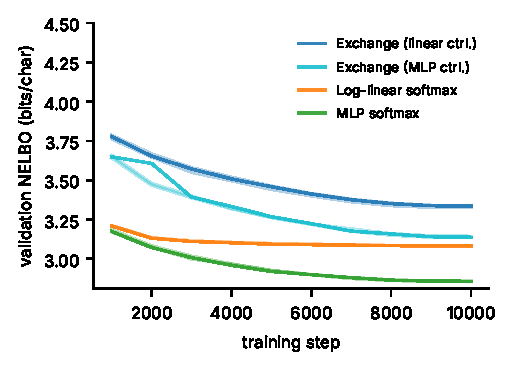
\includegraphics[width=\columnwidth]{figs/curves.pdf}
\caption{Validation NELBO during training (all seeds).}
\label{fig:curves}
\end{figure}
\begin{figure}[t]
\centering
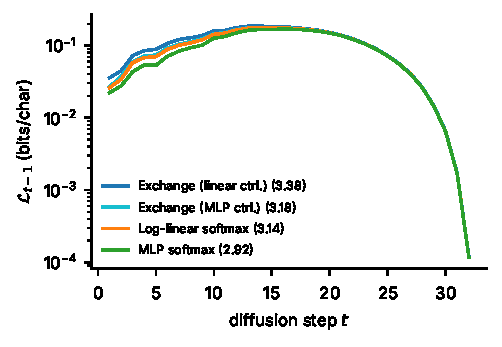
\includegraphics[width=\columnwidth]{figs/per_t.pdf}
\caption{Per-step contribution $\mathcal L_{t-1}$ to the test NELBO (seed 0; totals in the legend). The
exchange read-out loses at every noise level, with the largest relative gap at small $t$, where the
denoiser must copy $x_t$ with high confidence.}
\label{fig:per_t}
\end{figure}

\begin{figure}[t]
\centering\scriptsize
\resizebox{\columnwidth}{!}{%
\begin{tabular}{@{}r@{\;}l@{}}
$t$ & exchange denoiser (linear ctrl.), one sample\\
\midrule
32 & \texttt{flmi!jlfpaqbmhn,gzsu?fsul,k,'osexxjrx?awnjjh!'wzba,riyntpkzi?hdg}\\
28 & \texttt{ga.zejfwjdd~usm?laoscwagaxfstzeghpogn.glrbtnzjrd?fzblzt,?mk.gn.,}\\
24 & \texttt{m,kzfgf~jmd~~vmocao~cd,gzattozo!h'o!~.nvabyxzwr?!flgl,yu?ak.'nk,}\\
20 & \texttt{mmkzf~f~?mda~vr.oao~ag,ufztoozm!v'a!~.n!a~sxanrc!floleyjimb.'skw}\\
16 & \texttt{mmkwfcf~lvda~i..'ao~agyufttsgzj!v~aa~hn!a~s~anrn!flo,eetimb.'skw}\\
12 & \texttt{mpke~cf~lcda~i.~'a,~a~oufttssek!e~da~hn!a~'~an~,hfly,petimb.'s~w}\\
8 & \texttt{mpte~mf~lida~is~'a,~a~ountessekie~da~kn~a~'~an~thlly,petimb.'s~w}\\
4 & \texttt{mpte~sf~lida~is~'a,~a~qunte~sekre~dacre~a~b~an~thely~petimb.'s~w}\\
0 & \texttt{mpte~st~lipa~is~'a,~a~aunte~sekre~dacre~a~bjan~thely~metimb.'s~w}\\
\end{tabular}}
\caption{Measurement-based reverse diffusion from uniform noise ($t=32$) to text ($t=0$), shown every
4 steps.}
\label{fig:traj}
\end{figure}

\subsection{Ablations}
\begin{table}[t]
\centering\small
\caption{Ablations (seed 0, test NELBO in bits/char). $G$ = exchange gates, $D$ = layers.}
\label{tab:ablation}
\begin{tabular}{p{4.4cm}ccc}
\toprule
variant & $G$ & $D$ & NELBO\\
\midrule
\tabinput tables/ablation.tex 
\bottomrule
\end{tabular}
\end{table}
Table~\ref{tab:ablation} isolates the design choices.
(i) \emph{Depth.} One butterfly block (5 layers) gives $3.59$. Gains diminish beyond 3 blocks: 2 blocks
give $3.41$, 3 give $3.38$ and 6 give $3.36$.
(ii) \emph{Connectivity.} A 16-layer nearest-neighbour chain is below the light-cone depth and degrades
to $3.91$. A 48-layer chain ($3\times$ the gates) matches the butterfly ($3.35$).
(iii) \emph{Envelope.} Removing $J(t)$ costs $0.024$~bits/char.
(iv) \emph{Objective.} Training with the $x_0$ cross-entropy alone instead of the hybrid NELBO objective
costs $0.20$~bits/char.
(v) \emph{Features.} Without pair features the exchange model loses $0.27$ and the log-linear model
$0.28$, so the two read-outs use context features to a similar extent.
(vi) \emph{Re-uploading} with one 80-gate block per feature (16 blocks in sequence) reached $3.58$ in
half the steps. This matches the additive circuit with the same block size ($3.59$), but at
$16\times$ the circuit depth.

\subsection{Hardware noise}
\begin{figure*}[t]
\centering
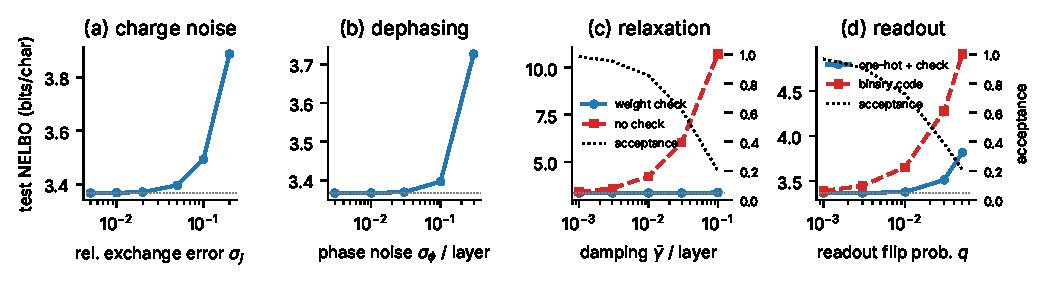
\includegraphics[width=0.92\textwidth]{figs/noise.pdf}
\caption{Test NELBO of the trained exchange denoiser (seed 0, 64 test windows, clean value 3.367 dotted)
under exactly simulated noise on all 32 qubits of every register.
(a) Quasi-static relative error of every exchange angle.
(b) Gaussian $Z$-phase per qubit per layer.
(c) Relaxation with qubit-dependent rates $\gamma_k\in[0.5,1.5]\bar\gamma$ per layer: Hamming-weight
check with post-selection (blue; dotted: acceptance) vs.\ no check, where a lost excitation is read as a
random token (red).
(d) Readout bit flips: one-hot register with weight check (blue; dotted: acceptance) vs.\ the same
distribution read out through a dense $\log_2V$-qubit binary code (red).}
\label{fig:noise}
\end{figure*}
Figure~\ref{fig:noise} shows the four noise channels of Sec.~\ref{sec:noise-theory}.
\emph{Charge noise}: a 2\% relative angle error costs $0.004$~bits/char and 5\% costs $0.03$.
\emph{Dephasing} up to $0.03$~rad per layer is negligible ($+0.003$).
\emph{Relaxation}: with the weight check the NELBO changes by less than $10^{-3}$~bits/char up to
$\bar\gamma=10^{-2}$ per layer, and rises by only $0.03$ at $\bar\gamma=0.1$, where 80\% of shots are
rejected. For uniform rates it is exactly unchanged ($3.3672$ at every $\gamma$), as predicted. Without the
check the same relaxation costs $0.07$ at $\bar\gamma=10^{-3}$ and $7.3$~bits/char at $0.1$.
\emph{Readout}: at $q=10^{-2}$ the one-hot register with weight check loses $0.012$ (acceptance 73\%),
while a binary code loses $0.29$. At $q=3\times10^{-2}$ the losses are $0.15$ and $0.91$.
